\documentclass[usletter]{article}
\usepackage{graphicx}
\usepackage{amsfonts}
\usepackage{amsthm}
\usepackage{amsmath}
\usepackage{amssymb}
\usepackage{scribe}
\usepackage[margin=1.5in]{geometry}

\begin{document}

\makeheader{Lowell Bander}{January 4, 2016}{1}{Deterministic Computation}

\noindent
During the first lecture of the course, we covered the formalisms for and semantics of the \emph{Turing Machine} (TM), a universal model of computation. We then proceeded to describe a TM which checks whether its input is a palindrome, so as to demonstrate how to construct a TM to solve an arbitrary problem.

During the second half of the lecture, we covered the notion of efficiency as it pertains to the time a TM takes to compute its output. Lastly, we showed that our standard definition of a TM can be used to simulate more complicated TM's, such as those with an enriched alphabet and those with bidirectional tapes. This last bit comes back to the notion that the Turing Machine is in fact a universal model of computation -- it can compute anything which is computable, even things which may seem to be computable only with more complex models of computation.

\section{Turing Machines Defined}

As mentioned in the preceding paragraphs, a Turing Machine (TM) is a universal model of computation. That is, it can simulate any computer algorithm, but this is not to say that it wouldn't be cumbersome to do so. For example, computing the first several numbers of the Fibonacci Sequence or creating an operating system would be much more easily done with languages such as Python and C, respectively, but both computations can be simulated with a TM. 

\begin{figure}[h!]
\begin{center}
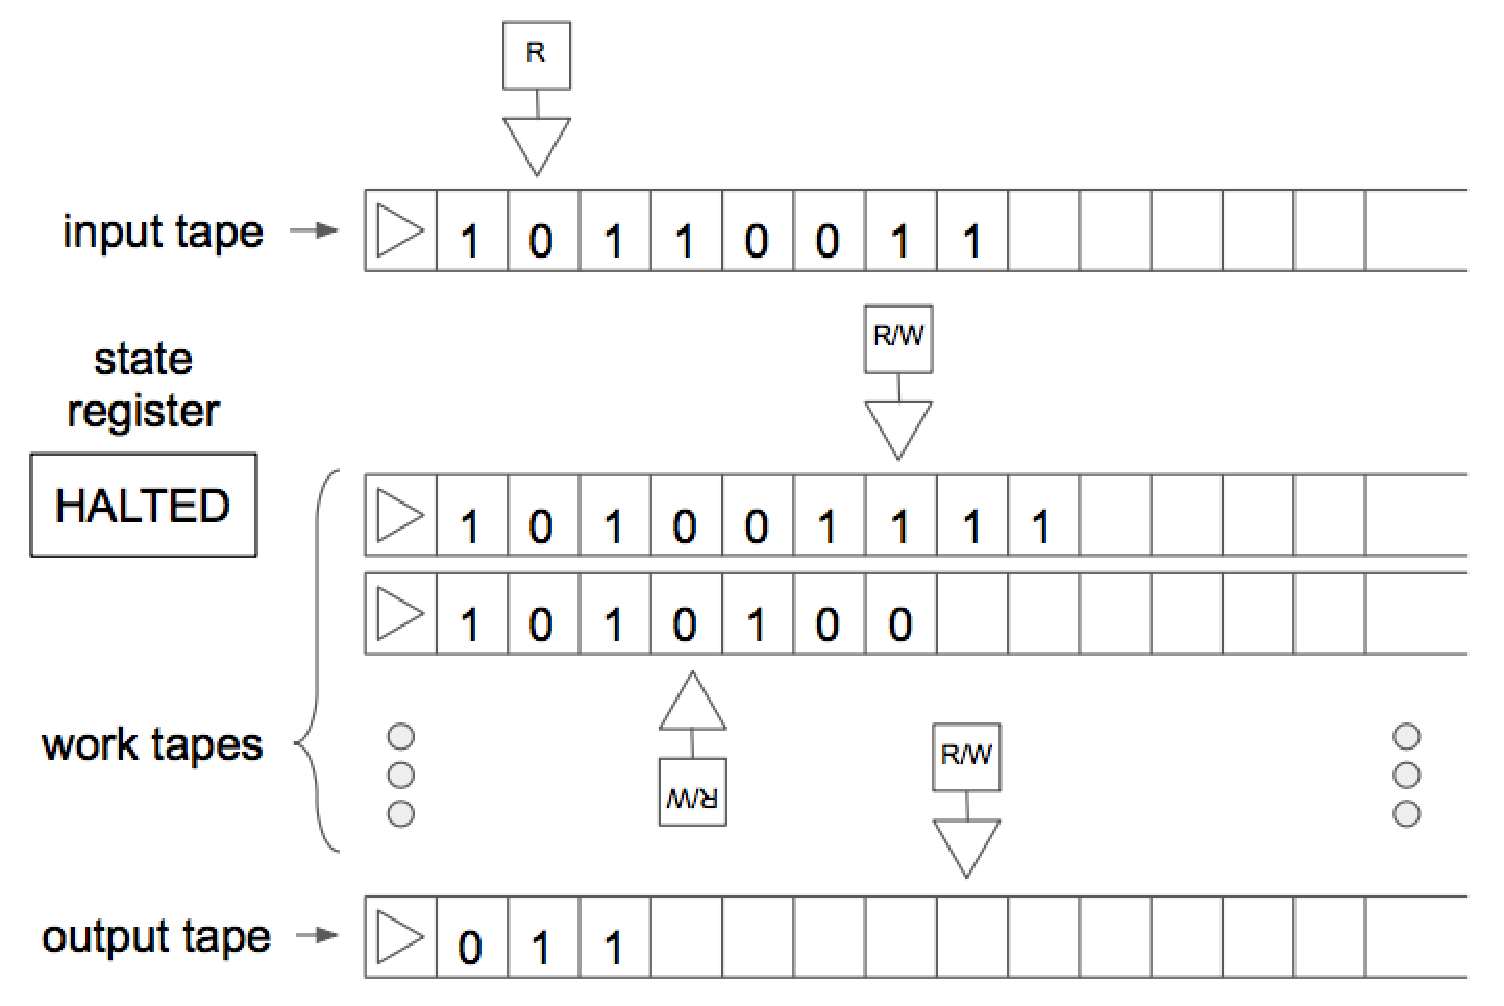
\includegraphics[width=\textwidth]{tm}
\end{center}
\caption{A standard Turing Machine.}
\label{fig:tm}
\end{figure}

As can be seen in Figure~\ref{fig:tm}, a TM consists of arbitrarily many tapes whose cells are capable of storing values. The first tape is known as the \emph{input tape}, and is used to represent the input to the TM, as its name suggests. The final tape in the TM is known as the \emph{output tape} and stores the result of the computation done by the TM. The remaining tapes are known as \emph{work tapes} and are used as a sort of scratch pad for the intermediate computation done by the TM.

The entities floating about the tapes in Figure~\ref{fig:tm} are \emph{tape heads}, all of which (except for the head of the input tape, which can only read) are capable of reading values from and writing values to the segment of the tape which they are pointing to at a given point in time. Additionally, all tape heads can either move to the left, move to the right, or stay put at each step in the computation performed by the TM.

Lastly, a TM has a a state register which is capable of storing, at any given time, one of the finitely many states available to the TM. In Figure~\ref{fig:tm}, the state register holds the value $HALTED$, which is the state a TM enters once it has finished computation.

Figure~\ref{fig:tm} and the accompanying description provides a useful visual intuition for the composition and behavior of a TM. However, it often proves useful to refer to the mathematical formalism of a TM, which is as follows. Formally, a TM is a tuple $(\Gamma, Q, \delta)$, such that $\Gamma$ is the alphabet of the TM, a finite set of symbols which has at minimum the subset $\{\Box, \rhd, 0, 1\}$, where $\Box$ is used for blank segments on the TM's tapes, and the $\rhd$ denotes the leftmost segment of a tape; $Q$ is a set of states which at minimum contains the states $START$ and $HALTED$, which are used, respectively, for the initial and final states of computation; and lastly $\delta$, the \emph{transition function} for the TM, which is used to determine what state to enter, what symbols to write to the tapes, and which direction (if any) to move each head, all based on the current state and the symbols beneath the every head of the TM. The transition function $\delta$ thus takes the following form: 

\begin{align}
\delta : Q \times \Gamma^k \rightarrow Q \times \Gamma^{k-1}\times \{\leftarrow, \cdot, \rightarrow\}^k
\end{align}
where $k$ is the number of total tapes in the TM. The superscript for $\Gamma$ in the domain and for the set $\{\leftarrow, \cdot, \rightarrow\}$ in the codomain is $k$ because all $k$ tapes are examined when determining the behavior of the TM in the current step, and all $k$ tapes can either move or stay put in any given step. Similarly, the superscript for $\Gamma$ in the codomain of $\delta$ is $k-1$ because all tapes have new values written to the segment currently pointed to by their respective heads except for the input tape, because its head is read-only.

\end{document}
